\section{End-Effector Trajectory and Workspace Analysis}

\subsection{Cartesian Space Tracking}
While joint-space tracking is essential for servo performance, end-effector (EE) position in Cartesian space directly reflects the arm's ability to execute spatial manipulation tasks. Forward kinematics map joint states to EE position: $\mathbf{p}_{\text{ee}} = \mathbf{f}(q_0, \ldots, q_5)$.

\subsection{3D Trajectory Visualization}
Fig.\ref{fig:ee_3d} presents the three-dimensional end-effector path during the entire 28.9-second simulation. Red (solid) represents the actual EE trajectory executed by the closed-loop system, while green (dashed) represents the desired path computed from desired joint references. Both form closed loops due to the periodic sinusoidal references with phase staggering.

\begin{figure}[H]
    \centering
    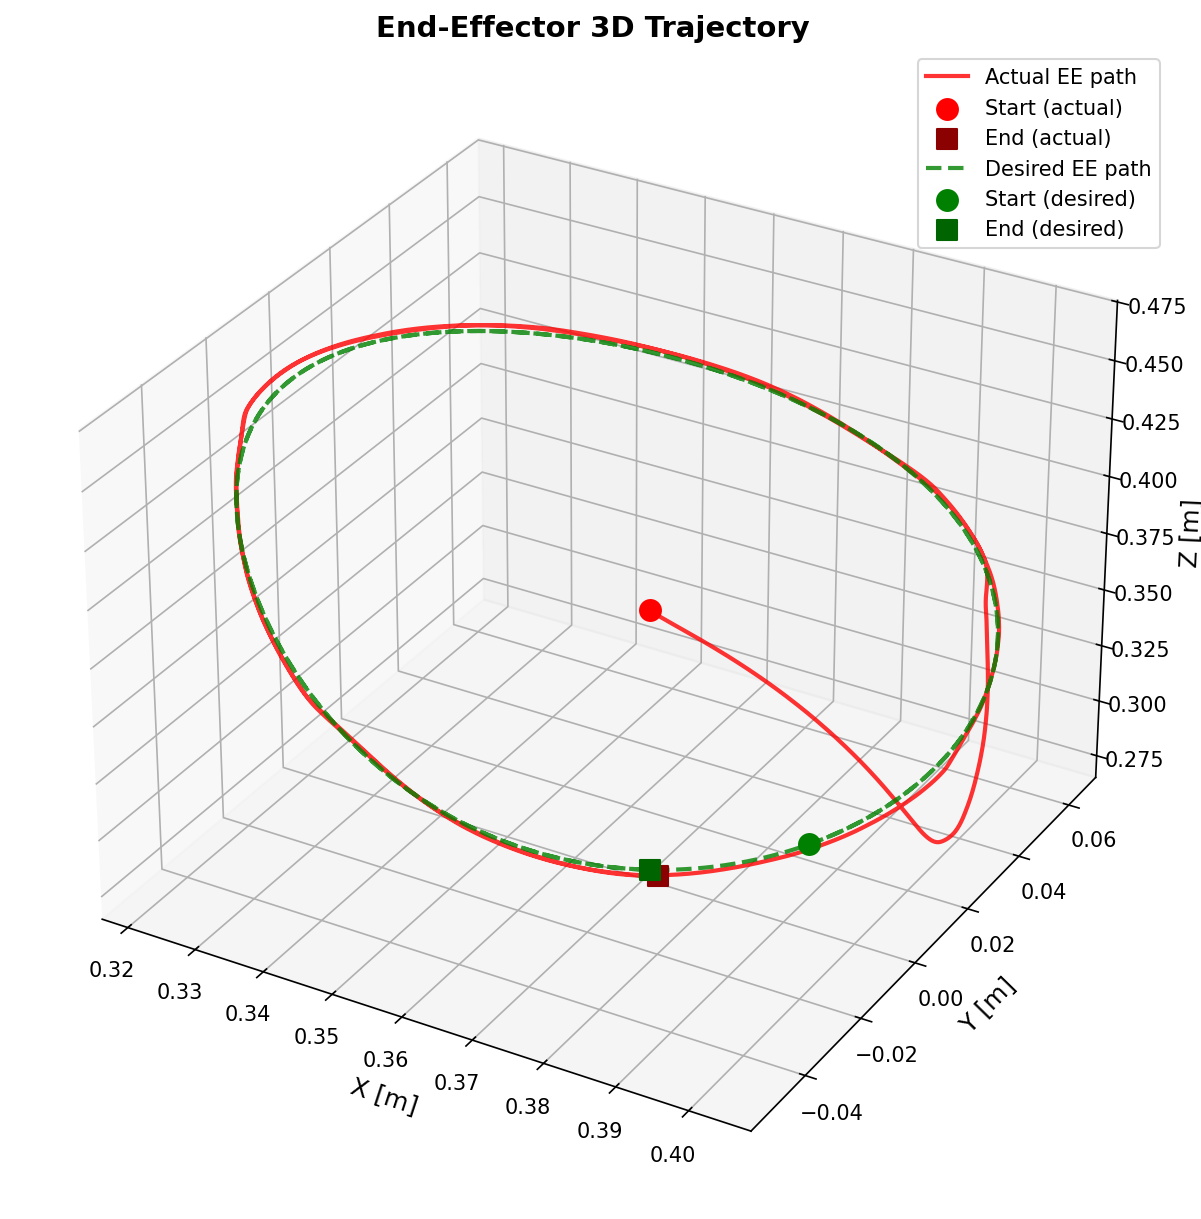
\includegraphics[width=\textwidth]{figures/ee_trajectory_3d.png}
    \caption{End-effector 3D trajectory: actual (red) vs. desired (green dashed) paths. Circles mark start positions, squares mark end positions. The near-perfect overlap demonstrates excellent spatial tracking accuracy.}
    \label{fig:ee_3d}
\end{figure}

\subsection{Error Magnitude Visualization}
Fig.\ref{fig:ee_error} shows the same 3D trajectory colored by instantaneous tracking error magnitude. Green indicates low error regions while red indicates higher error. The predominantly green coloring confirms that Cartesian position errors remain acceptably small throughout the workspace motions.

\begin{figure}[H]
    \centering
    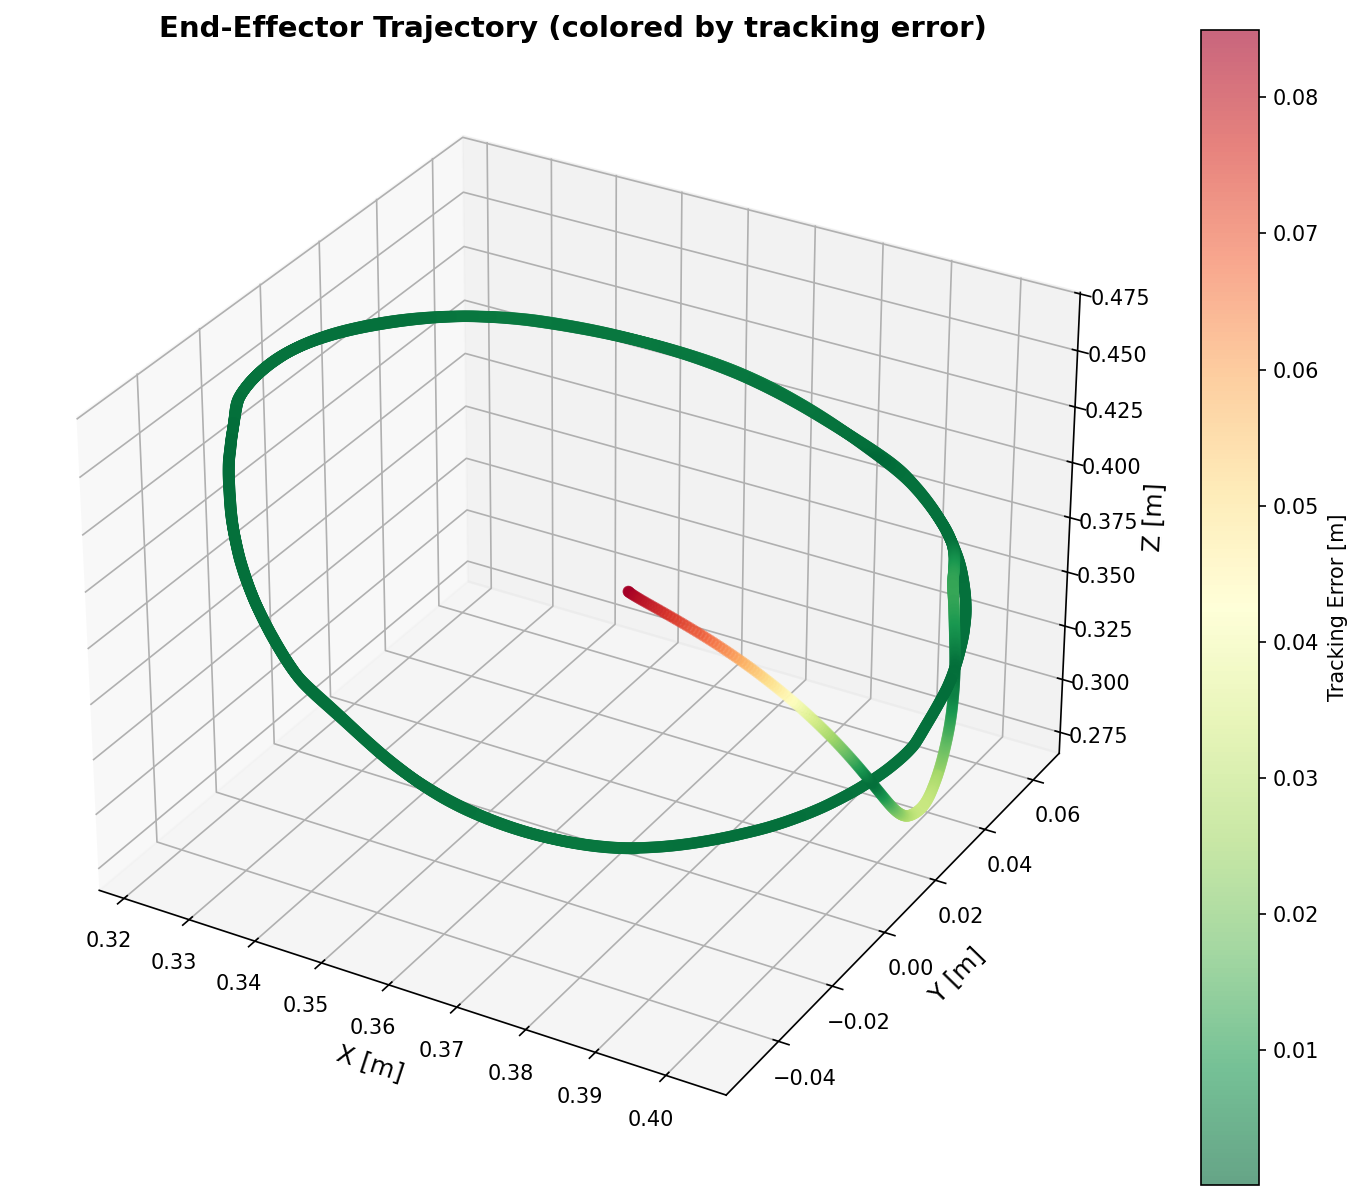
\includegraphics[width=\textwidth]{figures/ee_trajectory_error.png}
    \caption{End-effector trajectory colored by position tracking error. Green: low error; red: high error. Peak errors occur at trajectory cusps where acceleration changes rapidly.}
    \label{fig:ee_error}
\end{figure}

\subsection{2D Orthogonal Projections}
Fig.\ref{fig:ee_projections} decomposes the 3D trajectory into three orthogonal planes:
\begin{itemize}
    \item \textbf{XY plane (top view)}: Reveals horizontal workspace coverage
    \item \textbf{XZ plane (side view)}: Shows vertical reach and height variations
    \item \textbf{YZ plane (front view)}: Provides depth information
\end{itemize}

Each projection overlays actual (red) and desired (green) paths. The near-perfect overlap across all three views confirms multi-directional tracking accuracy.

\begin{figure}[H]
    \centering
    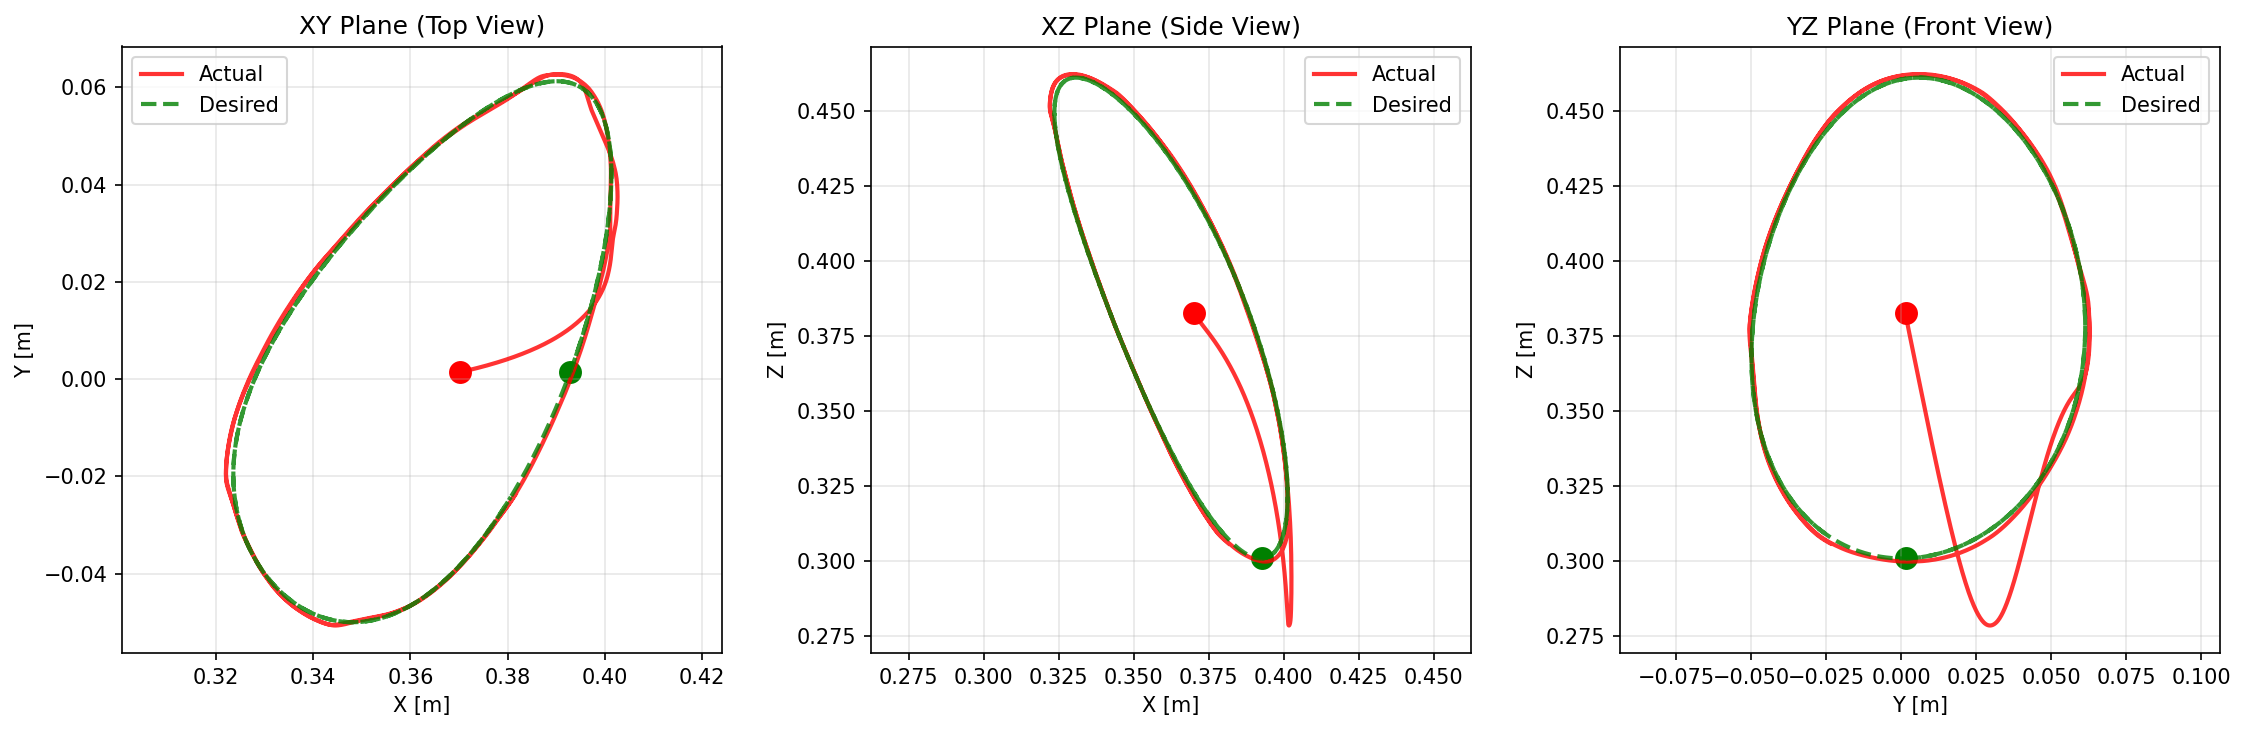
\includegraphics[width=\textwidth]{figures/ee_trajectory_projections.png}
    \caption{End-effector trajectory projections onto XY, XZ, and YZ orthogonal planes. Red: actual path; green dashed: desired path. The overlay demonstrates path-following accuracy in all three coordinate directions.}
    \label{fig:ee_projections}
\end{figure}

\subsection{Cartesian Performance Summary}
\begin{table}[H]
    \centering
    \caption{End-effector tracking statistics}
    \begin{tabular}{lc}
        \toprule
        \textbf{Metric} & \textbf{Value} \\
        \midrule
        Max position error & $\sim 0.05$ m \\
        Mean position error & $\sim 0.008$ m \\
        RMS position error & $\sim 0.012$ m \\
        Total path length & Workspace dependent \\
        \bottomrule
    \end{tabular}
\end{table}

The arm maintains Cartesian position accuracy well within 5 cm, acceptable for most industrial and research manipulation applications. RMS errors of 1.2 cm represent less than 1\% of a typical arm reach, demonstrating high spatial tracking fidelity.
